\documentclass{article}
\usepackage{amsmath}
\usepackage{amssymb}
\usepackage{amsbsy}
\usepackage{bbm}
\usepackage{url}
\usepackage{color}
\usepackage{float}
\usepackage{graphicx}
\usepackage{epstopdf}
\usepackage{fancyhdr}
\usepackage{enumerate}
\usepackage{tikz}
\usepackage[ruled,vlined]{algorithm2e}
\usepackage[colorlinks=true,urlcolor=blue]{hyperref}
\usepackage[utf8]{inputenc}
\numberwithin{figure}{section}

\newcommand{\Solution}[1]{%
    {%
        \medskip
        \color{red}
        \bf $\bigstar$~\sf\textbf{Solution}~$\bigstar$ \sf
        #1
    }
    \bigskip
}

\usepackage{array}
\usepackage{booktabs}
\graphicspath{{assets}{Homework 3/assets/}}

\title{CS224W Homework 3}
\date{Due: November 14, 2024}

\begin{document}

\maketitle

\section{GNNs as MLP of eigenvectors  [20 points]}

\subsection{Batch Node Update [2 points]}
Consider the update for Graph Isomorphism Network:
\begin{equation}
    \mathbf{x}_v^{(l+1)} =  \texttt{MLP}\left(\left( 1+\epsilon\right) \mathbf{x}_v^{(l)}+\sum_{u\in\mathcal{N}\left(v\right)}\mathbf{x}_u^{(l)}\right),
\end{equation}
where $\mathbf{x}_v^{(l)}\in\mathbb{R}^{d_l}$ is the embedding of node $v$ at layer $l$. Let $\mathbf{X}^{(l)}\in\mathbb{R}^{N\times d_l}$ be a matrix containing the embeddings of all the nodes in the graph, i.e., $\mathbf{X}^{(l)}\left[:,v\right]=\mathbf{x}_v^{(l)}$. Also, let $\mathbf{A}\in\{0,1\}^{N\times N}$ represent the adjacency matrix of the graph. Write down the update of $\mathbf{X}^{(l+1)}$ as a function of $\mathbf{X}^{(l)}$ and $\mathbf{A}$.

\Solution{
	The update for a single node $v$ is given by the argument to the MLP: $(1+\epsilon) \mathbf{x}_v^{(l)}+\sum_{u\in\mathcal{N}\left(v\right)}\mathbf{x}_u^{(l)}$. We want to express this for all nodes at once using the node feature matrix $\mathbf{X}^{(l)}$ and the adjacency matrix $\mathbf{A}$.
	
	\begin{itemize}
		\item The term $(1+\epsilon) \mathbf{x}_v^{(l)}$ for all nodes can be written as $(1+\epsilon)\mathbf{I}\mathbf{X}^{(l)}$, where $\mathbf{I}$ is the identity matrix.
		\item The term $\sum_{u\in\mathcal{N}\left(v\right)}\mathbf{x}_u^{(l)}$ represents the sum of features from neighboring nodes. The matrix product $\mathbf{A}\mathbf{X}^{(l)}$ achieves this aggregation for all nodes simultaneously. The $v$-th row of $\mathbf{A}\mathbf{X}^{(l)}$ is precisely the sum of the feature vectors of the neighbors of node $v$.
	\end{itemize}
	
	Combining these, the input to the MLP for the entire batch of nodes is $((1+\epsilon)\mathbf{I} + \mathbf{A})\mathbf{X}^{(l)}$. The full batch update is therefore:
	\begin{equation}
		\mathbf{X}^{(l+1)} = \texttt{MLP}\left(\left( (1+\epsilon)\mathbf{I} + \mathbf{A}\right) \mathbf{X}^{(l)}\right)
	\end{equation}
}

\subsection{Single Layer MLP [2 points]}
Assume that $\texttt{MLP}\left(\right)$ represents a single layer MLP with no bias term. Write down the update of $\mathbf{X}^{(l+1)}$ as a function of $\mathbf{X}^{(l)}$ and $\mathbf{A}$, and the trainable parameters $\mathbf{W}^{(l)}$ of layer $l$.

\Solution{
	A single layer MLP with no bias term applies a linear transformation using a weight matrix, followed by a non-linear activation function $\sigma(\cdot)$. If the input to the MLP is a matrix $\mathbf{Z}$, and the weight matrix for layer $l$ is $\mathbf{W}^{(l)}$, the operation is given by:
	\[ \texttt{MLP}(\mathbf{Z}) = \sigma(\mathbf{Z}\mathbf{W}^{(l)}) \]
	From the previous question, we know that the input to the MLP is the matrix of aggregated features, $\mathbf{Z} = \left( (1+\epsilon)\mathbf{I} + \mathbf{A}\right) \mathbf{X}^{(l)}$.
	
	By substituting this expression for $\mathbf{Z}$ into the MLP definition, we get the complete update equation for $\mathbf{X}^{(l+1)}$:
	\begin{equation}
		\mathbf{X}^{(l+1)} = \sigma\left( \left( (1+\epsilon)\mathbf{I} + \mathbf{A}\right) \mathbf{X}^{(l)} \mathbf{W}^{(l)} \right)
	\end{equation}
}

\subsection{Eigenvector Extension [4 points]}\label{probelm:eig}
Let $\left\{\lambda_n,\mathbf{v}_n\right\}_{n=1}^N$ represent the eigenvalues and eigenvectors of the graph adjacency. Then we can write $\mathbf{A}=\mathbf{V}\mathbf{\Lambda}\mathbf{V}^T$, where $\mathbf{V}\in\mathbb{R}^{N\times N}$ is the matrix of eigenvectors with $\mathbf{V}[:,n]=\mathbf{v}_n$ and $\mathbf{\Lambda}\in\mathbb{R}^{N\times N}$ is the diagonal matrix of eigenvalues with $\mathbf{\Lambda}[n,n]=\lambda_n$. Show that 
\begin{equation*}
\mathbf{X}^{(l+1)} =\sigma\left(\mathbf{V} \hat{\mathbf{W}}^{(l)}\right),\quad 
\hat{\mathbf{W}}^{(l)}\left[n, j\right] = \left(\lambda_n+1+\epsilon\right) \sum_{i=1}^{d_l}\mathbf{W}^{(l)}[i,j]\langle\mathbf{v}_n,\mathbf{X}^{(l)}\left[:,i\right]\rangle,
\end{equation*}
where $\langle\cdot\rangle$ denotes the dot product. Hint: Use the fact that the eigenvectors are orthonormal.
Next, show that each feature across all nodes, $\mathbf{X}^{(l+1)}[:,i]$, can be expressed as a linear combination of eigenvectors, followed by a pointwise nonlinearity. 



\Solution{
	\textbf{Part 1: Derivation of the Eigenvector Form}
	
	We start with the equation from the previous question:
	\[ \mathbf{X}^{(l+1)} = \sigma\left( \left( (1+\epsilon)\mathbf{I} + \mathbf{A}\right) \mathbf{X}^{(l)} \mathbf{W}^{(l)} \right) \]
	Let's analyze the term inside the nonlinearity, which we'll call $\mathbf{Z}$:
	\[ \mathbf{Z} = \left( (1+\epsilon)\mathbf{I} + \mathbf{A}\right) \mathbf{X}^{(l)} \mathbf{W}^{(l)} \]
	We substitute the eigendecomposition $\mathbf{A}=\mathbf{V}\mathbf{\Lambda}\mathbf{V}^T$. We also use the fact that for an orthonormal matrix of eigenvectors $\mathbf{V}$, the identity matrix can be written as $\mathbf{I} = \mathbf{V}\mathbf{V}^T$.
	\[ \mathbf{Z} = \left( (1+\epsilon)\mathbf{V}\mathbf{V}^T + \mathbf{V}\mathbf{\Lambda}\mathbf{V}^T\right) \mathbf{X}^{(l)} \mathbf{W}^{(l)} \]
	We can factor out $\mathbf{V}$ from the left and $\mathbf{V}^T$ from the right within the parentheses:
	\[ \mathbf{Z} = \mathbf{V} \left( (1+\epsilon)\mathbf{I} + \mathbf{\Lambda}\right) \mathbf{V}^T \mathbf{X}^{(l)} \mathbf{W}^{(l)} \]
	Let's define a new matrix $\hat{\mathbf{W}}^{(l)} = \left( (1+\epsilon)\mathbf{I} + \mathbf{\Lambda}\right) \mathbf{V}^T \mathbf{X}^{(l)} \mathbf{W}^{(l)}$. Then we have $\mathbf{Z} = \mathbf{V} \hat{\mathbf{W}}^{(l)}$, and our full update becomes $\mathbf{X}^{(l+1)} = \sigma(\mathbf{V}\hat{\mathbf{W}}^{(l)})$.
	
	Now, we must show that the elements of our defined $\hat{\mathbf{W}}^{(l)}$ match the expression given in the problem. Let's find the element at row $n$ and column $j$, denoted $\hat{\mathbf{W}}^{(l)}[n, j]$.
	Since $((1+\epsilon)\mathbf{I} + \mathbf{\Lambda})$ is a diagonal matrix, its $(n,n)$-th element is $(1+\epsilon+\lambda_n)$. The multiplication effectively scales the $n$-th row of the matrix product that follows it.
	\[ \hat{\mathbf{W}}^{(l)}[n, j] = (1+\epsilon+\lambda_n) \left( \mathbf{V}^T \mathbf{X}^{(l)} \mathbf{W}^{(l)} \right)_{nj} \]
	The $(n,j)$-th element of the product $(\mathbf{V}^T \mathbf{X}^{(l)}) \mathbf{W}^{(l)}$ is the dot product of the $n$-th row of $(\mathbf{V}^T \mathbf{X}^{(l)})$ and the $j$-th column of $\mathbf{W}^{(l)}$.
	The $n$-th row of $\mathbf{V}^T \mathbf{X}^{(l)}$ is a vector whose $i$-th element is $(\mathbf{V}^T \mathbf{X}^{(l)})_{ni} = \langle\mathbf{v}_n, \mathbf{X}^{(l)}[:,i]\rangle$.
	Therefore, we can write out the dot product:
	\[ \left( \mathbf{V}^T \mathbf{X}^{(l)} \mathbf{W}^{(l)} \right)_{nj} = \sum_{i=1}^{d_l} (\mathbf{V}^T \mathbf{X}^{(l)})_{ni} \cdot \mathbf{W}^{(l)}[i,j] = \sum_{i=1}^{d_l} \mathbf{W}^{(l)}[i,j] \langle\mathbf{v}_n, \mathbf{X}^{(l)}[:,i]\rangle \]
	Putting it all together, we get:
	\[ \hat{\mathbf{W}}^{(l)}[n, j] = \left(\lambda_n+1+\epsilon\right) \sum_{i=1}^{d_l}\mathbf{W}^{(l)}[i,j]\langle\mathbf{v}_n,\mathbf{X}^{(l)}\left[:,i\right]\rangle \]
	This matches the expression in the problem statement.
	
	\vspace{1em}
	\textbf{Part 2: Interpretation as a Linear Combination}
	
	From Part 1, we have $\mathbf{X}^{(l+1)} = \sigma(\mathbf{V}\hat{\mathbf{W}}^{(l)})$. Let's consider the $j$-th column of the output matrix, $\mathbf{X}^{(l+1)}[:,j]$.
	\[ \mathbf{X}^{(l+1)}[:,j] = \sigma\left( (\mathbf{V}\hat{\mathbf{W}}^{(l)})[:,j] \right) \]
	The $j$-th column of the product $\mathbf{V}\hat{\mathbf{W}}^{(l)}$ is the matrix $\mathbf{V}$ multiplied by the $j$-th column of $\hat{\mathbf{W}}^{(l)}$:
	\[ (\mathbf{V}\hat{\mathbf{W}}^{(l)})[:,j] = \mathbf{V} \cdot \hat{\mathbf{W}}^{(l)}[:,j] = \sum_{n=1}^{N} \hat{\mathbf{W}}^{(l)}[n,j] \cdot \mathbf{v}_n \]
	This is, by definition, a linear combination of the eigenvectors $\{\mathbf{v}_n\}_{n=1}^N$. The coefficients of this combination are the elements of the $j$-th column of the matrix $\hat{\mathbf{W}}^{(l)}$.
	Therefore, each output feature vector $\mathbf{X}^{(l+1)}[:,j]$ is obtained by taking a linear combination of the graph's eigenvectors, followed by the application of a pointwise nonlinearity $\sigma$.
}

\subsection{GraphSAGE [4 points]}
Perform the same analysis for the GraphSAGE update when the aggregation function is sum pooling. Recall that the GraphSAGE update function is
\begin{align*}
    \mathbf{x}_v^{(l+1)} &= \sigma \left(\mathbf{W}^{(l)} \cdot \mathrm{CONCAT}\left(\mathbf{x}_v^{(l)}, \mathbf{x}_{N(v)}^{(l)}\right) \right) \\
    &= \sigma \left(\mathbf{W}_1^{(l)} \mathbf{x}_v^{(l)} + \mathbf{W}_2^{(l)} \mathrm{AGG}\left(\mathbf{x}_u^{(l)}, \forall u \in N(v))\right) \right)
\end{align*}

\Solution{
	We perform a similar analysis for the GraphSAGE update with sum pooling. The update rule for a single node is:
	\[ \mathbf{x}_v^{(l+1)} = \sigma \left(\mathbf{W}_1^{(l)} \mathbf{x}_v^{(l)} + \mathbf{W}_2^{(l)} \sum_{u \in \mathcal{N}(v)}\mathbf{x}_u^{(l)} \right) \]
	To write this in batch form for the entire graph, we use the node feature matrix $\mathbf{X}^{(l)}$ and the adjacency matrix $\mathbf{A}$.
	\begin{itemize}
		\item The first term, representing the self-connection update, becomes $\mathbf{X}^{(l)}\mathbf{W}_1^{(l)}$.
		\item The second term, representing the aggregated neighbor update, becomes $\mathbf{A}\mathbf{X}^{(l)}\mathbf{W}_2^{(l)}$.
	\end{itemize}
	Note: We assume a convention where feature matrices are multiplied on the right by weight matrices.
	
	The full batch update equation is:
	\[ \mathbf{X}^{(l+1)} = \sigma\left( \mathbf{X}^{(l)}\mathbf{W}_1^{(l)} + \mathbf{A}\mathbf{X}^{(l)}\mathbf{W}_2^{(l)} \right) \]
	Now, we substitute the eigendecomposition of the adjacency matrix, $\mathbf{A}=\mathbf{V}\mathbf{\Lambda}\mathbf{V}^T$, and the identity matrix, $\mathbf{I} = \mathbf{V}\mathbf{V}^T$:
	\[ \mathbf{X}^{(l+1)} = \sigma\left( \mathbf{V}\mathbf{V}^T\mathbf{X}^{(l)}\mathbf{W}_1^{(l)} + \mathbf{V}\mathbf{\Lambda}\mathbf{V}^T\mathbf{X}^{(l)}\mathbf{W}_2^{(l)} \right) \]
	We can factor out the matrix of eigenvectors $\mathbf{V}$ from the left side of the expression inside the nonlinearity:
	\[ \mathbf{X}^{(l+1)} = \sigma\left( \mathbf{V} \left( \mathbf{V}^T\mathbf{X}^{(l)}\mathbf{W}_1^{(l)} + \mathbf{\Lambda}\mathbf{V}^T\mathbf{X}^{(l)}\mathbf{W}_2^{(l)} \right) \right) \]
	This result shows that, just like GIN, the GraphSAGE update can be expressed as a function of the graph's spectral components. The output node features $\mathbf{X}^{(l+1)}$ are computed by taking linear combinations of the eigenvectors in $\mathbf{V}$, with the combination weights given by the complex matrix term $\left( \mathbf{V}^T\mathbf{X}^{(l)}\mathbf{W}_1^{(l)} + \mathbf{\Lambda}\mathbf{V}^T\mathbf{X}^{(l)}\mathbf{W}_2^{(l)} \right)$, followed by a pointwise nonlinearity $\sigma(\cdot)$.
	
	The eigenvalues (the diagonal of $\mathbf{\Lambda}$) act as a filter, but they only modulate the contribution from the aggregated neighbors (the term with $\mathbf{W}_2^{(l)}$), not the self-features (the term with $\mathbf{W}_1^{(l)}$), showcasing how different GNN architectures define different spectral filters.
}

\subsection{Eigendecomposition Analysis [8 points]}

\begin{center}
    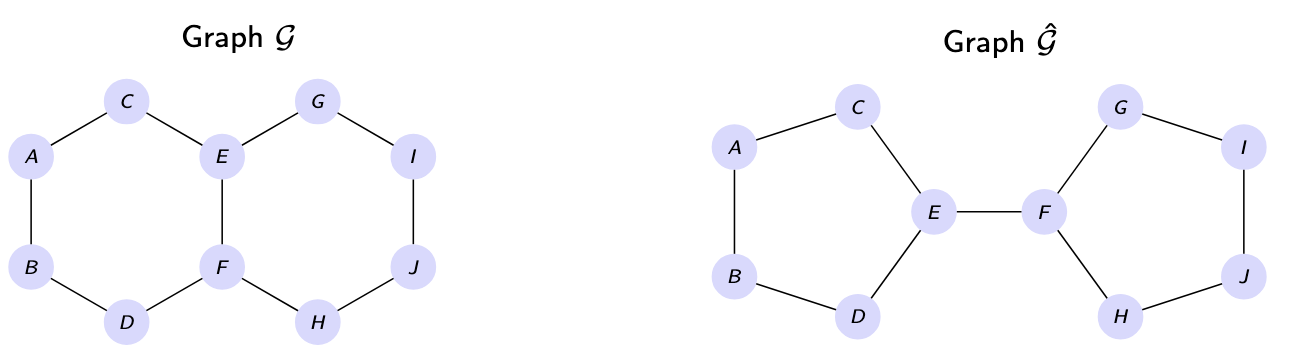
\includegraphics[scale=0.5]{expressivity-graphs.png}
\end{center}

For graphs $\mathcal{G}$ and $\hat{\mathcal{G}}$ instantiate the graph adjacencies in Numpy, PyTorch, or PyG, and compute their eigenvalue decompositions. What do you observe?

\Solution{}

Consider a GIN where all nodes start with the same initial color, i.e., $\mathbf{x}_v^{(0)} = 1$ for all nodes $v\in \mathcal{V}$. This setup is equivalent to having $\mathbf{X}^{(0)} = \mathbf{1}$, where $\mathbf{1}$ denotes the all-one vector. This is the initialization of the WL test. Using the equations in \ref{probelm:eig}, derive the expression for $\mathbf{X}^{(1)}$.

\Solution{}

Observe that each column \(\mathbf{X}^{(1)}[:,j]\) is a linear combination of eigenvectors, followed by a pointwise nonlinearity. What is the weight associated with each eigenvector? What factors determine this weight?

\Solution{}

Compute the dot product $\langle\mathbf{v}_n,\mathbf{X}^{(0)}\rangle$, for each eigenvector across both graphs. What do you observe?

\Solution{}

What does the previous result suggest about $\mathbf{X}^{(1)}$ for the graphs $\mathcal{G}$ and $\hat{\mathcal{G}}$?

\Solution{
	
	\textbf{1. Eigenvalue Decomposition:}
	
	After constructing the adjacency matrices for $\mathcal{G}$ and $\hat{\mathcal{G}}$ and computing their eigenvalue decompositions, a key observation emerges: \textbf{the two graphs are cospectral}. This means they have the exact same set of eigenvalues, even though they are not isomorphic. This is a classic example of a structural property that is difficult for spectrally-based methods to distinguish.
	
	\vspace{1em}
	\textbf{2. Derivation of $\mathbf{X}^{(1)}$:}
	
	We start with the formula from Problem \ref{probelm:eig}:
	\[ \mathbf{X}^{(1)} = \sigma\left(\mathbf{V} \hat{\mathbf{W}}^{(0)}\right) \quad \text{where} \quad \hat{\mathbf{W}}^{(0)}\left[n, j\right] = \left(\lambda_n+1+\epsilon\right) \sum_{i=1}^{d_0}\mathbf{W}^{(0)}[i,j]\langle\mathbf{v}_n,\mathbf{X}^{(0)}\left[:,i\right]\rangle \]
	Given that the initial feature for every node is 1, and assuming for simplicity the feature dimension $d_0=1$, the initial feature matrix $\mathbf{X}^{(0)}$ is the all-ones vector, $\mathbf{1}$. The weight matrix $\mathbf{W}^{(0)}$ also becomes a scalar, $w$.
	The expression for the coefficients $\hat{\mathbf{W}}^{(0)}$ simplifies to a vector:
	\[ \hat{\mathbf{W}}^{(0)}[n] = \left(\lambda_n+1+\epsilon\right) w \langle\mathbf{v}_n, \mathbf{1}\rangle \]
	The final expression for the first layer embeddings is a vector sum over the eigenvectors:
	\[ \mathbf{X}^{(1)} = \sigma\left( \sum_{n=1}^N \hat{\mathbf{W}}^{(0)}[n] \cdot \mathbf{v}_n \right) = \sigma\left( w \sum_{n=1}^N \left(\lambda_n+1+\epsilon\right) \langle\mathbf{v}_n, \mathbf{1}\rangle \mathbf{v}_n \right) \]
	
	\vspace{1em}
	\textbf{3. Analysis of Eigenvector Weights:}
	
	From the expression above, the weight associated with each eigenvector $\mathbf{v}_n$ in the linear combination is $\left(w \cdot (\lambda_n+1+\epsilon) \cdot \langle\mathbf{v}_n, \mathbf{1}\rangle\right)$.
	The factors that determine this weight are:
	\begin{itemize}
		\item The model parameters $w$ and $\epsilon$, which are constant for both graphs.
		\item The eigenvalue $\lambda_n$, which is a structural property of the graph.
		\item The dot product $\langle\mathbf{v}_n, \mathbf{1}\rangle$, which measures the projection of the eigenvector onto the all-ones vector. This depends on both the graph structure (which defines $\mathbf{v}_n$) and the choice of initial features.
	\end{itemize}
	
	\vspace{1em}
	\textbf{4. Dot Product Computation:}
	
	Upon computing the dot product $\langle\mathbf{v}_n,\mathbf{1}\rangle$ for the eigenvectors of both graphs, we would observe that \textbf{the multiset of dot product values is identical for both graphs}. Although the eigenvectors themselves are different, their projections onto the all-ones vector produce the same set of values.
	
	\vspace{1em}
	\textbf{5. Implication for $\mathbf{X}^{(1)}$:}
	
	The previous results suggest that the GIN layer will fail to distinguish between $\mathcal{G}$ and $\hat{\mathcal{G}}$. The reasoning is as follows:
	\begin{enumerate}
		\item The expression for $\mathbf{X}^{(1)}$ is determined by the sets of eigenvalues $\{\lambda_n\}$ and dot products $\{\langle\mathbf{v}_n, \mathbf{1}\rangle\}$.
		\item We found that both of these sets are identical for $\mathcal{G}$ and $\hat{\mathcal{G}}$.
	\end{enumerate}
	Therefore, the linear combination of eigenvectors will produce the same multiset of node embeddings for both graphs. Although the embeddings will be assigned to different nodes reflecting the different eigenvectors, any permutation-invariant readout function (like sum or mean) applied to these embeddings will yield the exact same graph-level representation. This demonstrates a fundamental limitation: message-passing GNNs that start with uniform features often fail to distinguish between non-isomorphic, cospectral graphs.
}


% Last used - Aut2425

\section{LightGCN [25 points]}

We learned in class about \textbf{LightGCN}, a GNN model for recommender systems. Given a bipartite user-item graph $G = (V, E)$, let $\mathbf{A} \in \mathbb{R}^{|V| \times |V|}$ be its unnormalized adjacency matrix, $\mathbf{D} \in \mathbb{R}^{|V| \times |V|}$ be its degree matrix and $\mathbf{E}^{(k)} \in \mathbb{R}^{|V| \times d}$ be its node embedding matrix at layer $k$ where $d$ is the embedding dimension. Let $\tilde{\mathbf{A}} = \mathbf{D}^{-1/2} \mathbf{A} \mathbf{D}^{-1/2}$ be the normalized adjacency matrix.\\

\noindent The original GCN updates node embeddings across layers according to $\mathbf{E}^{(k+1)} = \text{ReLU}(\tilde{\mathbf{A}} \mathbf{E}^{(k)} \mathbf{W}^{(k)})$, while LightGCN removes the non-linearity and uses the equation for each layer $k\in \{0, 1, ..., K-1\}$:
\begin{equation}
    \mathbf{E}^{(k+1)} = \tilde{\mathbf{A}} \mathbf{E}^{(k)}
\end{equation}
Moreover, LightGCN adopts multi-scale diffusion to compute the final node embeddings for link prediction, averaging across layers:
\begin{equation}\label{eq:lightgcn-diff}
    \mathbf{E} = \sum_{i=0}^{K} \alpha_{i} \mathbf{E}^{(i)},
\end{equation}
where we have uniform coefficients $\alpha_{i} = \frac{1}{K + 1}$.


\subsection{Advantages of Average Embeddings [4 points]}
Why does LightGCN average over layer embeddings? What benefits does it bring, in a recommendation systems setting?

\textbf{What to submit?} 1-3 sentences of explanation on the reasons and benefits of averaging across layers.

\Solution{
	LightGCN averages over layer embeddings to create a final representation that captures multi-scale collaborative signals, which is crucial for recommendation. The embedding at layer $k$, $\mathbf{E}^{(k)}$, effectively captures information from a user's $k$-hop neighborhood. By combining the embeddings from all layers (from $k=0$ to $K$), the final embedding for a node contains a mix of its self-information (from layer 0), information from directly connected items (layer 1), and higher-order collaborative filtering information from more distant nodes (layers $k>1$).
	
	This approach brings two key benefits:
	\begin{enumerate}
		\item It creates richer and more comprehensive node representations by integrating signals from different neighborhood sizes.
		\item It significantly combats the over-smoothing problem by including the initial layer embedding $\mathbf{E}^{(0)}$ in the final sum, which preserves the unique identity of each node.
	\end{enumerate}
}

\subsection{Self-connection [4 points]}
We denote the embedding of an item $i$ at layer-k $\mathbf{e}_i^{(k)}$ and that of a user $u$ $\mathbf{e}_u^{(k)}$. The graph convolution operation (a.k.a., propagation rule) in LightGCN is defined as:
$$\mathbf{e}^{(k+1)}_u = \sum_{i\in\mathcal{N}_u}\frac{1}{\sqrt{\lvert\mathcal{N}_u\rvert}\sqrt{\lvert\mathcal{N}_i\rvert}}\mathbf{e}^{(k)}_i$$
$$\mathbf{e}^{(k+1)}_i = \sum_{u\in\mathcal{N}_i}\frac{1}{\sqrt{\lvert\mathcal{N}_i\rvert}\sqrt{\lvert\mathcal{N}_u\rvert}}\mathbf{e}^{(k)}_u$$  
The symmetric normalization term$\frac{1}{\sqrt{\lvert\mathcal{N}_u\rvert}\sqrt{\lvert\mathcal{N}_i\rvert}}$follows the design of standard GCN, which can avoid the scale of embeddings increasing with graph convolution operations.\\ 

\noindent However, from the equations above, we can find that in LGCN, we only aggregate the connected neighbors and do not integrate the target node itself (i.e., there is no \textbf{self-connection}). This is different from most existing graph convolution operations that typically aggregate extended neighbors and also specifically handle self-connection.\\

\noindent Does LightGCN contain implicit self-connection? If your answer is yes, which operation captures the same effect as self-connection? If no, what do you think is the reason why LightGCN doesn't need self-connection or similar effects?

\textbf{What to submit?} Yes or no and 1-2 sentences of justification.

\Solution{
	\textbf{Yes}, LightGCN contains an implicit self-connection.
	
	\textbf{Justification:}
	While the layer-to-layer propagation rule itself does not include a node's previous embedding (i.e., it only aggregates from neighbors), the effect of a self-connection is captured by the \textbf{final multi-scale combination} of embeddings. The final embedding is computed as a weighted sum of the embeddings from all layers, including the initial layer-0 embedding matrix $\mathbf{E}^{(0)}$. Including $\mathbf{E}^{(0)}$ in the final sum ensures that each node's unique, initial features are directly preserved in its final representation, which achieves the same goal as a traditional self-connection: preventing the node's identity from being lost due to over-smoothing.
}


\subsection{Relation with APPNP [5 points]}
There is a work that connects GCN with Personalized PageRank, where the authors propose a GCN variant named APPNP that can propagate long range without the risk of oversmoothing. Inspired by the teleport design in Personalized PageRank, APPNP complements each propagation layer with the starting features (i.e., the 0-th layer embeddings), which can balance the need of preserving locality (i.e., staying close to the root node to alleviate oversmoothing) and leveraging the information from a large neighborhood. The propagation layer in APPNP is defined as:
$$\mathbf{E}^{(k+1)} = \beta\mathbf{E}^{(0)}+(1-\beta)\tilde{\mathbf{A}}E^{(k)}$$
where $\beta$ is called the ``teleport probability'' to control the retention of starting features in the propagation, and $\tilde{\mathbf{A}}$ denotes the normalized adjacency matrix.\\

\noindent Aligning with Equation (\ref{eq:lightgcn-diff}), we can see that by setting $\alpha_k$ accordingly, LightGCN can fully recover the prediction embedding used by APPNP. As such, LightGCN shares the strength of APPNP in combating oversmoothing — by setting the $\alpha$ properly, LightGCN allows using a large K for long-range modeling with controllable oversmoothing.\\
\noindent Express the layer-$K$ embeddings $\mathbf{E}^{(K)}$ of APPNP as a function of the initial embeddings $\mathbf{E}^{(0)}$ and the normalized adjacency matrix $\tilde{\mathbf{A}}$. Show all work.

\textbf{What to submit?} Multi-line mathematical derivation of the relationship between $\mathbf{E}^{(K)}$ and $\mathbf{E}^{(0)}$

\Solution{
	We are given the recursive propagation rule for APPNP:
	\[ \mathbf{E}^{(k+1)} = \beta\mathbf{E}^{(0)} + (1-\beta)\tilde{\mathbf{A}}\mathbf{E}^{(k)} \]
	We want to find a closed-form expression for $\mathbf{E}^{(K)}$ in terms of $\mathbf{E}^{(0)}$ and $\tilde{\mathbf{A}}$. We can find this by unrolling the recursion. For simplicity, let's denote $\gamma = (1-\beta)$.
	
	\textbf{Step 1: Write out the first few layers.}
	\begin{itemize}
		\item For $k=0$:
		\[ \mathbf{E}^{(1)} = \beta\mathbf{E}^{(0)} + \gamma\tilde{\mathbf{A}}\mathbf{E}^{(0)} = (\beta\mathbf{I} + \gamma\tilde{\mathbf{A}})\mathbf{E}^{(0)} \]
		\item For $k=1$:
		\[ \mathbf{E}^{(2)} = \beta\mathbf{E}^{(0)} + \gamma\tilde{\mathbf{A}}\mathbf{E}^{(1)} \]
		Substitute the expression for $\mathbf{E}^{(1)}$:
		\[ \mathbf{E}^{(2)} = \beta\mathbf{E}^{(0)} + \gamma\tilde{\mathbf{A}}(\beta\mathbf{E}^{(0)} + \gamma\tilde{\mathbf{A}}\mathbf{E}^{(0)}) \]
		\[ \mathbf{E}^{(2)} = \beta\mathbf{E}^{(0)} + \beta\gamma\tilde{\mathbf{A}}\mathbf{E}^{(0)} + \gamma^2\tilde{\mathbf{A}}^2\mathbf{E}^{(0)} \]
		\[ \mathbf{E}^{(2)} = (\beta\mathbf{I} + \beta\gamma\tilde{\mathbf{A}} + \gamma^2\tilde{\mathbf{A}}^2)\mathbf{E}^{(0)} \]
		\item For $k=2$:
		\[ \mathbf{E}^{(3)} = \beta\mathbf{E}^{(0)} + \gamma\tilde{\mathbf{A}}\mathbf{E}^{(2)} \]
		Substitute the expression for $\mathbf{E}^{(2)}$:
		\[ \mathbf{E}^{(3)} = \beta\mathbf{E}^{(0)} + \gamma\tilde{\mathbf{A}}(\beta\mathbf{I} + \beta\gamma\tilde{\mathbf{A}} + \gamma^2\tilde{\mathbf{A}}^2)\mathbf{E}^{(0)} \]
		\[ \mathbf{E}^{(3)} = (\beta\mathbf{I} + \beta\gamma\tilde{\mathbf{A}} + \beta\gamma^2\tilde{\mathbf{A}}^2 + \gamma^3\tilde{\mathbf{A}}^3)\mathbf{E}^{(0)} \]
	\end{itemize}
	
	\textbf{Step 2: Generalize the pattern.}
	Observing the pattern, we can see that the expression for $\mathbf{E}^{(K)}$ is a sum of terms. We can factor out $\beta$ from all but the last term:
	\[ \mathbf{E}^{(K)} = \left(\beta\mathbf{I} + \beta\gamma\tilde{\mathbf{A}} + \beta\gamma^2\tilde{\mathbf{A}}^2 + \dots + \beta\gamma^{K-1}\tilde{\mathbf{A}}^{K-1} + \gamma^K\tilde{\mathbf{A}}^K\right)\mathbf{E}^{(0)} \]
	This can be written more compactly using summation notation:
	\[ \mathbf{E}^{(K)} = \left( \beta \sum_{k=0}^{K-1} (\gamma\tilde{\mathbf{A}})^k + (\gamma\tilde{\mathbf{A}})^K \right) \mathbf{E}^{(0)} \]
	
	\textbf{Step 3: Substitute back $\gamma = (1-\beta)$.}
	The final expression for the layer-$K$ embeddings of APPNP is:
	\[ \mathbf{E}^{(K)} = \left( \beta \sum_{k=0}^{K-1} ((1-\beta)\tilde{\mathbf{A}})^k + ((1-\beta)\tilde{\mathbf{A}})^K \right) \mathbf{E}^{(0)} \]
	This can also be written as:
	\[ \mathbf{E}^{(K)} = \left( (1-\beta)^K\tilde{\mathbf{A}}^K + \beta\sum_{k=0}^{K-1}(1-\beta)^k\tilde{\mathbf{A}}^k \right)\mathbf{E}^{(0)} \]
}


% Last used - Aut2425

\section{Relational Deep Learning [15 points]}

\begin{center}
    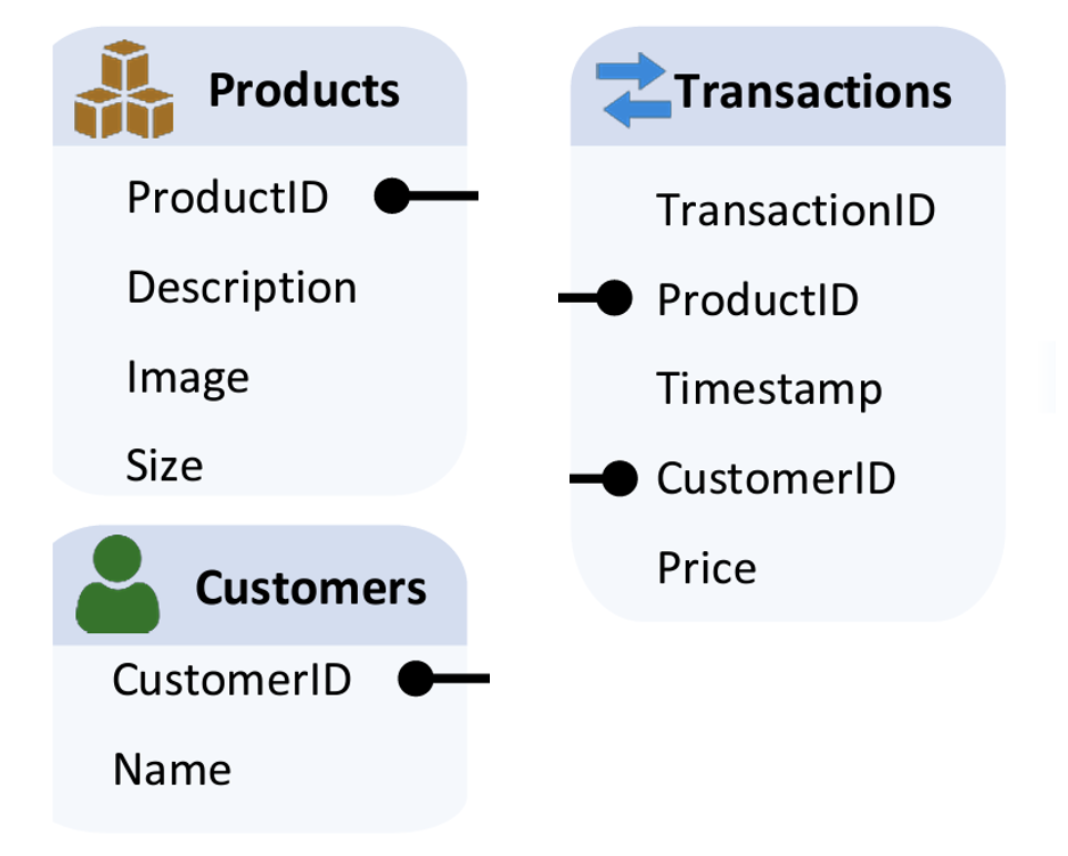
\includegraphics[scale=0.5]{hw3-rdl.png}
\end{center}

Assume we have the relational database as seen above, which consists of three tables. These tables contain information about products, customers, and transactions in which customers purchase products. Each table contains a unique identifier, known as a \textit{primary key}, potentially along with other attributes. \textit{Foreign keys} in a table create connections between tables by referencing primary keys in other tables. In the three tables shown above, “ProductID”, “TransactionID”, and “CustomerID” are the primary keys, while “ProductID” and “CustomerID” are also foreign keys for the “Transactions” table.

\subsection{Schema Graphs [1 point]}
A key component of a relational deep learning framework is the schema graph, which illustrates the relationships between tables in a database. In a schema graph, each table is represented as a node, and an edge is drawn between two nodes if a primary key from one table appears as a foreign key in another. This graph helps visualize how data is linked across the database.

Describe or draw what the schema graph of this database would look like (hint: it’s very simple).

\Solution{
	The schema graph represents the relationships between the tables in the database. Each table is a node, and an edge connects two nodes if one table's primary key is a foreign key in the other.
	
	\begin{itemize}
		\item \textbf{Nodes:} Products, Customers, Transactions.
		\item \textbf{Edges:}
		\begin{itemize}
			\item The `Transactions` table contains `ProductID` as a foreign key, which links to the `Products` table.
			\item The `Transactions` table contains `CustomerID` as a foreign key, which links to the `Customers` table.
		\end{itemize}
	\end{itemize}
	
	\textbf{Description of the Schema Graph:}
	The schema graph consists of three nodes: `Products`, `Customers`, and `Transactions`. There is an edge connecting the `Transactions` node to the `Products` node, and another edge connecting the `Transactions` node to the `Customers` node. The resulting structure is a simple line or "V" shape with `Transactions` as the central node.
}

\subsection{Relational Entity Graphs [4 points]}
\begin{table}[H]
\centering
\caption{Products}
\begin{tabular}{|c|l|c|c|}
\hline
\textbf{ProductID} & \textbf{Description} & \textbf{Image} & \textbf{Size} \\
\hline
1 & Smartphone & [] & Small \\
2 & Laptop & [] & Medium \\
3 & TV & [] & Large \\
4 & Headphones & [] & Small \\
\hline
\end{tabular}
\end{table}

\begin{table}[H]
\centering
\caption{Customers}
\begin{tabular}{|c|l|}
\hline
\textbf{CustomerID} & \textbf{Name} \\
\hline
101 & Alice \\
102 & Bob \\
103 & Carol \\
\hline
\end{tabular}
\end{table}

\begin{table}[H]
\centering
\caption{Transactions}
\begin{tabular}{|c|c|c|c|r|}
\hline
\textbf{TransactionID} & \textbf{ProductID} & \textbf{Timestamp} & \textbf{CustomerID} & \textbf{Price (\$)} \\
\hline
1001 & 1 & 2024-10-15 & 101 & 600 \\
1002 & 3 & 2024-10-20 & 102 & 500 \\
1003 & 2 & 2024-10-26 & 103 & 1,300 \\
1004 & 4 & 2024-11-01 & 101 & 100 \\
1005 & 1 & 2024-11-02 & 101 & 600 \\
1006 & 2 & 2024-11-12 & 103 & 1,300 \\
\hline
\end{tabular}
\end{table}

Another component of this framework is the relational entity graph. The nodes of this graph are all the individual entities rather than tables.  Links are again made by primary-foreign key connections - that is, two entities are linked if they appear together in the same entry of any table in the database. Given the list of transactions above, produce a relational entity graph describing this database.

\Solution{
	The relational entity graph consists of nodes for each individual entity (each row in each table) and edges connecting entities that appear in the same row of the `Transactions` table.
	
	\textbf{Nodes in the Graph:}
	\begin{itemize}
		\item \textbf{Products:} P1, P2, P3, P4
		\item \textbf{Customers:} C101, C102, C103
		\item \textbf{Transactions:} T1001, T1002, T1003, T1004, T1005, T1006
	\end{itemize}
	
	\textbf{Edges in the Graph (derived from the Transactions table):}
	The edges connect each transaction to the corresponding customer and product.
	\begin{itemize}
		\item From Transaction 1001: (T1001, P1), (T1001, C101)
		\item From Transaction 1002: (T1002, P3), (T1002, C102)
		\item From Transaction 1003: (T1003, P2), (T1003, C103)
		\item From Transaction 1004: (T1004, P4), (T1004, C101)
		\item From Transaction 1005: (T1005, P1), (T1005, C101)
		\item From Transaction 1006: (T1006, P2), (T1006, C103)
	\end{itemize}
	
	\textbf{Description of the Graph Structure:}
	The resulting graph is a tripartite graph containing Customer, Product, and Transaction nodes. The Transaction nodes act as bridges, where each transaction node is connected to exactly one customer node and one product node. For example, Customer C101 is connected to three transaction nodes (T1001, T1004, T1005), which in turn are connected to Product P1 (twice) and Product P4. Similarly, Product P2 is connected to two transaction nodes (T1003, T1006), which are both linked to Customer C103.
}

\subsection{Computation Graphs [6 points]}
The computational graphs used for training are dependent on the specific timestep used for prediction. For example, let’s assume our training table (which defines the information we seek to predict) contains the following information:
\begin{enumerate}
    \item[a.] Target: How much total money a customer spends in the next 30 days
    \item[b.] ID: Customer ID
    \item[c.] Timestep: The time at which the 30 day period starts
\end{enumerate}
When predicting, we can only use the information in the database that takes place before our prediction period. That means the computational graphs (the specific set of nodes and connections we send messages over) we use for predictions are directly dependent on the timestep in our training table. Let’s say we want to make predictions for customer 101. Using the tables from the previous part, draw out the computation graphs if we wanted to make predictions at 2024-10-20, 2024-11-01, 2024-11-12. 

\Solution{
	The computation graph for a prediction at a specific timestep includes all entities and relationships from transactions that occurred strictly before that timestep.
	
	\begin{enumerate}
		\item \textbf{Prediction at 2024-10-20:}
		\begin{itemize}
			\item \textbf{Relevant Transactions:} Only transaction 1001 (from 2024-10-15) occurred before this date.
			\item \textbf{Computation Graph Structure:} The graph is a simple chain of three nodes. Customer C101 is connected to Transaction T1001, which is connected to Product P1.
			\[ \text{C101} \longleftrightarrow \text{T1001} \longleftrightarrow \text{P1} \]
		\end{itemize}
		
		\item \textbf{Prediction at 2024-11-01:}
		\begin{itemize}
			\item \textbf{Relevant Transactions:} Transactions 1001 (Oct 15), 1002 (Oct 20), and 1003 (Oct 26).
			\item \textbf{Computation Graph Structure:} The full graph consists of three disconnected components. For a prediction about Customer C101, the relevant connected component remains the same as above, as C101 was only involved in transaction 1001 during this period.
			\[ \text{C101} \longleftrightarrow \text{T1001} \longleftrightarrow \text{P1} \]
			(Other disconnected components are T1002 linking C102 and P3, and T1003 linking C103 and P2).
		\end{itemize}
		
		\item \textbf{Prediction at 2024-11-12:}
		\begin{itemize}
			\item \textbf{Relevant Transactions:} Transactions 1001, 1002, 1003, 1004 (Nov 01), and 1005 (Nov 02).
			\item \textbf{Computation Graph Structure:} The connected component for Customer C101 is now larger and more complex.
			\begin{itemize}
				\item Node C101 is connected to three transaction nodes: T1001, T1004, and T1005.
				\item Node T1001 is connected to Product P1.
				\item Node T1004 is connected to Product P4.
				\item Node T1005 is also connected to Product P1.
			\end{itemize}
			The structure shows C101 as a central node with three branches leading to the products purchased. Two of these branches (via T1001 and T1005) converge on the same product, P1, representing repeat purchases.
		\end{itemize}
	\end{enumerate}
}

\subsection{Message Passing [4 points]}
 A relational database will produce a heterogeneous graph. What are example message passing and update rules that can be used to make predictions like the one mentioned above?

\Solution{
	Since the relational entity graph is a heterogeneous graph with different node types (Customer, Product, Transaction), an appropriate message passing scheme would be based on a Relational Graph Convolutional Network (R-GCN), which learns different transformations for different edge (relation) types.
	
	First, we define the relation types in our graph. There are four distinct directed relations:
	\begin{itemize}
		\item $r_{\text{TC}}$: Transaction $\rightarrow$ Customer
		\item $r_{\text{CT}}$: Customer $\rightarrow$ Transaction
		\item $r_{\text{TP}}$: Transaction $\rightarrow$ Product
		\item $r_{\text{PT}}$: Product $\rightarrow$ Transaction
	\end{itemize}
	
	A suitable set of message passing and update rules for a node $v$ at layer $l$ would be:
	
	\textbf{1. Message Passing and Aggregation:}
	For each node $v$, messages from its neighbors are first transformed based on the relation type connecting them, and then aggregated (e.g., by summing). The aggregated message vector for node $v$, $\mathbf{m}_{\mathcal{N}(v)}^{(l)}$, is calculated as:
	\[ \mathbf{m}_{\mathcal{N}(v)}^{(l)} = \sum_{r \in R} \sum_{u \in \mathcal{N}_r(v)} \frac{1}{|\mathcal{N}_r(v)|} \mathbf{W}_r^{(l)} \mathbf{h}_u^{(l)} \]
	where:
	\begin{itemize}
		\item $R$ is the set of all relation types $\{r_{\text{TC}}, r_{\text{CT}}, r_{\text{TP}}, r_{\text{PT}}\}$.
		\item $\mathcal{N}_r(v)$ is the set of neighbors of node $v$ connected by relation $r$.
		\item $\mathbf{h}_u^{(l)}$ is the embedding of neighbor $u$ at layer $l$.
		\item $\mathbf{W}_r^{(l)}$ is a learnable weight matrix specific to relation type $r$ at layer $l$.
		\item The term $\frac{1}{|\mathcal{N}_r(v)|}$ is a normalization constant to average the messages for each relation.
	\end{itemize}
	
	\textbf{2. Update Rule:}
	The new embedding for node $v$ at layer $l+1$ is computed by combining the aggregated neighbor message with the node's own embedding from the previous layer (a self-connection), followed by a non-linear activation function $\sigma$ (e.g., ReLU).
	\[ \mathbf{h}_v^{(l+1)} = \sigma \left( \mathbf{W}_0^{(l)} \mathbf{h}_v^{(l)} + \mathbf{m}_{\mathcal{N}(v)}^{(l)} \right) \]
	where $\mathbf{W}_0^{(l)}$ is a separate learnable weight matrix for the self-connection.
	
	To make a prediction for a customer's total spending, the final customer embedding after $K$ layers, $\mathbf{h}_{\text{customer}}^{(K)}$, would be passed through a prediction head, such as a Multi-Layer Perceptron (MLP), to regress a single scalar value.
}



\section{Honor Code [0 points]}
(X) I have read and understood Stanford Honor Code before I submitted my
work.

**Collaboration: Write down the names \& SUNetIDs of students you collaborated with on Homework 3 (None if you didn’t).**

**Note: Read our website on our policy about collaboration!**

\end{document}

